% !TeX root = ../../tesis.tex

% -----------------------------------------------------------------------
\subsection{Tiempo de Viaje Promedio \texorpdfstring{($T$)}{(T)}}
\label{subsec:tiempo-viaje}
% -----------------------------------------------------------------------

\textbf{Fuente principal:} \citet{aldous2019optimal}

\subsubsection{Definición y Fundamentación}

El Tiempo de Viaje Promedio es la métrica de desempeño global del sistema y el
criterio de optimización central del modelo. \citet{aldous2019optimal} plantean
que el criterio de optimalidad en el diseño de redes de transporte consiste en
minimizar el tiempo promedio de viaje entre pares de puntos elegidos
independientemente según su distribución en el territorio.

De manera particularmente relevante para la hipótesis central de este trabajo,
\citet{aldous2019optimal} demuestran analíticamente que, a medida que la
longitud total de la red aumenta, ocurre una transición brusca en un valor
crítico $L_c$ en el que aparece un bucle o anillo en la topología óptima de la
red. Esto implica que, para redes de transporte a escala metropolitana, la
incorporación de un corredor perimetral ---como el Anillo Periférico
propuesto--- no solo es viable, sino que constituye la forma
\textit{óptima esperada} de expansión de la red una vez superado cierto umbral
de longitud total. Este resultado teórico provee el sustento matemático directo
para la hipótesis de investigación.

\subsubsection{Fórmula}

\begin{equation}
    T = \frac{1}{N \cdot (N-1)} \sum_{i \neq j} t_{ij}
    \label{eq:tiempo-promedio}
\end{equation}

Donde:
\begin{itemize}
    \item $T$ = Tiempo de Viaje Promedio global de la red, en minutos.
    \item $N$ = Número total de nodos (estaciones y paradas) del grafo.
    \item $t_{ij}$ = Tiempo mínimo de viaje desde el nodo $i$ hasta el nodo $j$,
    calculado mediante el algoritmo de \dijkstra{} sobre el grafo ponderado,
    en minutos. Incluye tiempo en vehículo + tiempo de caminata + tiempo de
    espera en andén + penalización por transbordo.
\end{itemize}

El indicador $T$ se calculará en dos escenarios: la red metropolitana actual y
la red con la incorporación del Anillo Periférico. La diferencia
$\Delta T = T_{\text{actual}} - T_{\text{propuesto}}$ constituye la medida
cuantitativa principal de la viabilidad de la propuesta.

\begin{figure}[H]
    \centering
    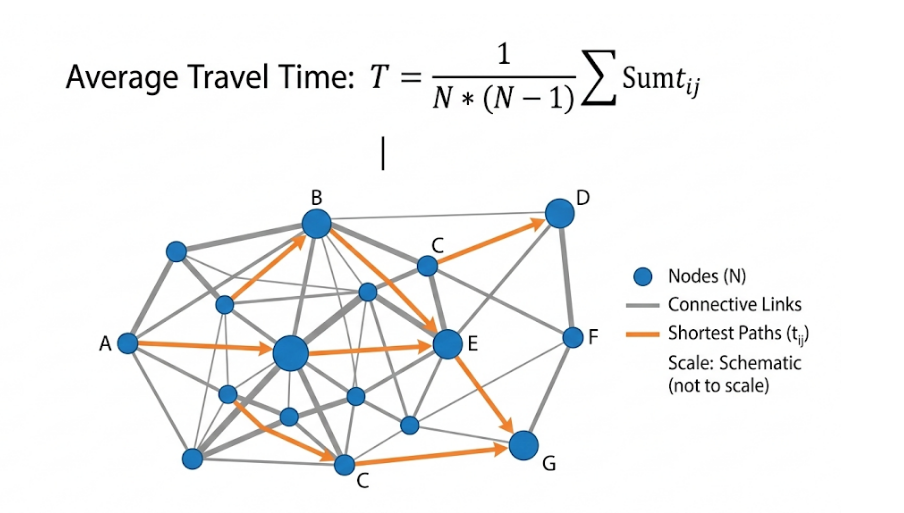
\includegraphics[width=0.72\textwidth]{Figures/Cap3/TiempoViajePromedio.png}
    \caption[Diagrama del indicador de Tiempo de Viaje Promedio $T$]{Red con
    nodos $N$, aristas grises (enlaces conectores) y caminos mínimos
    $t_{ij}$ (caminos más cortos) resaltados.}
    \label{fig:indicador-T}
    \fuentefigura{Elaboración propia con base en \citet{aldous2019optimal}.}
\end{figure}


\subsubsection{Ejemplo Práctico: \cdmx{} y Zona Metropolitana}

\begin{table}[H]
    \centering
    \caption{Estimaciones del indicador $T$ por escenario.}
    \label{tab:tiempo-promedio}
    \begin{tabularx}{\textwidth}{X r}
        \toprule
        \textbf{Escenario} & \textbf{$T$ estimado} \\
        \midrule
        Red radial actual (sin anillo) & $\approx 85$ minutos \\
        Red con propuesta del Anillo Periférico & $\approx 65$ minutos \\
        Reducción $\Delta T$ & $\approx 20$ min ($-24\%$) \\
        \bottomrule
    \end{tabularx}
\end{table}

La implementación computacional de referencia para este indicador se encuentra
en el \autoref{anx:indicadores-implementacion} (§\ref{anx:impl-tiempo}). La
proyección de paradas geográficas a nodos del grafo previa al cálculo de
$t_{ij}$ se describe en §\ref{subsubsec:snapping}.

El indicador $T$ es el criterio de optimización central de la investigación,
referenciado explícitamente en los Objetivos Específicos 2 y 5 (§
\ref{subsec:obj-especificos}). La diferencia
$\Delta T = T_{\text{actual}} - T_{\text{propuesto}}$ es la cifra que cuantifica
el beneficio global del escenario hipotético anillar; el resultado teórico de
\citet{aldous2019optimal} sobre la transición brusca en $L_c$ provee el sustento
matemático de por qué ese $\Delta T$ debe ser positivo para una red
metropolitana del tamaño de la \zmvm{}.
